\section{Proceso de paralelización}\label{proceso-par}

A la hora de paralelizar un programa seguimos cuatro pasos:

\begin{itemize}
	\item Descomponer el programa en tareas independientes.
	\item Asignar tareas a procesos y hebras.
	\item Redactar el código paralelo como vimos en \S\ref{herramientas-progpar}.
	\item Evaluar las prestaciones que ofrece la paralelización.
\end{itemize}

Estos cuatro pasos deben seguirse secuencialmente, y de la evaluación podemos volver a cualquiera de los tres anteriores en función de los errores que hayamos detectado o dar por finalizada la paralelización del programa.

\subsection{Descomposición en tareas independientes}\label{descomposicion-tareas-independientes}

Para descomponer un programa secuencial en tareas independientes debemos llevar a cabo un análisis de dependencias de datos entre las diferentes funciones en las que se divide y, dentro de éstas, entre los diferentes bloques que las componen.
Al hacer esto podemos crear un grafo de dependencias que ilustre qué funciones y bloques pueden ejecutarse paralelamente en cada momento.

\begin{figure}[h]
\begin{center}
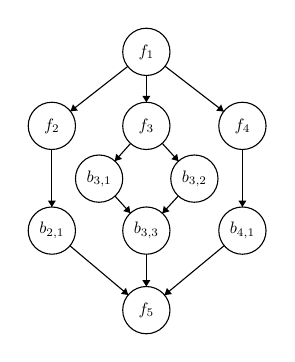
\begin{tikzpicture}[scale=0.1, every node/.style={scale=0.6}]
\tikzstyle{every node}+=[inner sep=0pt]
\draw [black] (27.4,-10.3) circle (3);
\draw (27.4,-10.3) node {$f_4$};
\draw [black] (3.2,-10.3) circle (3);
\draw (3.2,-10.3) node {$f_2$};
\draw [black] (15.2,-0.9) circle (3);
\draw (15.2,-0.9) node {$f_1$};
\draw [black] (15.2,-10.3) circle (3);
\draw (15.2,-10.3) node {$f_3$};
\draw [black] (9.2,-17) circle (3);
\draw (9.2,-17) node {$b_{3,1}$};
\draw [black] (21.3,-17) circle (3);
\draw (21.3,-17) node {$b_{3,2}$};
\draw [black] (15.2,-23.6) circle (3);
\draw (15.2,-23.6) node {$b_{3,3}$};
\draw [black] (27.4,-23.6) circle (3);
\draw (27.4,-23.6) node {$b_{4,1}$};
\draw [black] (3.2,-23.6) circle (3);
\draw (3.2,-23.6) node {$b_{2,1}$};
\draw [black] (15.2,-33.7) circle (3);
\draw (15.2,-33.7) node {$f_5$};
\draw [black] (12.84,-2.75) -- (5.56,-8.45);
\fill [black] (5.56,-8.45) -- (6.5,-8.35) -- (5.88,-7.56);
\draw [black] (15.2,-3.9) -- (15.2,-7.3);
\fill [black] (15.2,-7.3) -- (15.7,-6.5) -- (14.7,-6.5);
\draw [black] (17.58,-2.73) -- (25.02,-8.47);
\fill [black] (25.02,-8.47) -- (24.7,-7.58) -- (24.08,-8.38);
\draw [black] (17.22,-12.52) -- (19.28,-14.78);
\fill [black] (19.28,-14.78) -- (19.11,-13.85) -- (18.37,-14.53);
\draw [black] (13.2,-12.53) -- (11.2,-14.77);
\fill [black] (11.2,-14.77) -- (12.11,-14.5) -- (11.36,-13.84);
\draw [black] (11.22,-19.22) -- (13.18,-21.38);
\fill [black] (13.18,-21.38) -- (13.01,-20.45) -- (12.27,-21.12);
\draw [black] (19.26,-19.2) -- (17.24,-21.4);
\fill [black] (17.24,-21.4) -- (18.15,-21.15) -- (17.41,-20.47);
\draw [black] (27.4,-13.3) -- (27.4,-20.6);
\fill [black] (27.4,-20.6) -- (27.9,-19.8) -- (26.9,-19.8);
\draw [black] (3.2,-13.3) -- (3.2,-20.6);
\fill [black] (3.2,-20.6) -- (3.7,-19.8) -- (2.7,-19.8);
\draw [black] (5.5,-25.53) -- (12.9,-31.77);
\fill [black] (12.9,-31.77) -- (12.61,-30.87) -- (11.97,-31.64);
\draw [black] (25.09,-25.51) -- (17.51,-31.79);
\fill [black] (17.51,-31.79) -- (18.45,-31.66) -- (17.81,-30.89);
\draw [black] (15.2,-26.6) -- (15.2,-30.7);
\fill [black] (15.2,-30.7) -- (15.7,-29.9) -- (14.7,-29.9);
\end{tikzpicture}

\end{center}
\caption{Grafo de dependencias entre las tareas de un programa}
\end{figure}

Por ejemplo, tengamos el siguiente código para aproximar el número pi:

\begin{lstlisting}[language=C]
int main (int argc, char ** argv) {
	double ancho,
	       sum = 0,
	       x;
	int intervalos;

	intervalos = atoi(argv[1]);
	ancho      = 1.0 / (double) intervalos;

	for (int i=0; i<intervalos; i++) {
		x    = (i + 0.5) * ancho;
		sum += 4.0 / (1.0 + x * x);
	}

	sum *= ancho;
}
\end{lstlisting}

En él, identificamos tres bloques principales:

\begin{itemize}
	\item Declaración e inicialización de variables.
	\item Cálculo de la aproximación en bucle.
	\item Ajuste final de la aproximación.
\end{itemize}

Mientras que el primer y último bloque son indivisibles, el segundo podemos dividirlo en $n$ tareas que se ejecuten paralelamente para $n$ intervalos usados en la aproximación, de forma que cada uno de los valores de \code{i} en el bucle se ejecute de forma paralela a los otros.

\subsection{Asignación de tareas a procesos y hebras}\label{asignacion-tareas-procheb}

En esta fase distinguimos dos tipos de asignación de las tareas:

\begin{itemize}
	\item\textbf{Planificación:} Agrupación de las tareas en hebras.
	\item\textbf{\textit{Mapping}:} Asignación de las hebras a núcleos o procesadores.
\end{itemize}

La granularidad de la carga asignada a los procesos y hebras depende del número de núcleos o procesadores y del tiempo de comunicación y sincronización frente al tiempo de cálculo de cada hebra y procesador.
Para que la ejecución de unas tareas no dependa de esperar el resultado de otras, se busca un \textbf{equilibrado de la carga} (\textit{load balancing}) teniendo en cuenta que todas trabajen con un número lo más equitativo posible de datos y ejecuten un código lo más similar posible.
Este equilibrado depende de la homogeneidad y uniformidad de la arquitectura sobre la que se trabaja y sobre la descomposición del programa realizada anteriormente.

La asignación de las tareas a cada una de las hebras se puede hacer de forma estática, asignando las hebras en tiempo de compilación, o dinámica, en cuyo caso la asignación se hace en tiempo de ejecución.
En esta última diferentes ejecuciones del programa pueden dar lugar a asignaciones de las tareas sobre diferentes hebras o procesadores.
Ambas asignaciones se pueden hacer de forma explícitas por el programador o de forma implícita por la herramienta de programación utilizada.

El \textit{mapping} de las hebras se suele dejar al SO, que lo implementa mediante un sistema llamado \textit{light-weight process}.
También puede hacerse por el entorno o el sistema en tiempo de ejecución (\textit{runtime system}) o explicitarse por el programador.

Debemos tener en cuenta que dividir el programa en más tareas paralelas que procesadores requiere una carga de trabajo de cambio de contexto para los procesadores que ralentiza la ejecución global del programa y que la creación de hebras conlleva un tiempo de ejecución que puede ser mayor que el tiempo de ejecución secuencial al sumarlo a la ejecución paralela de las tareas.

\begin{lstlisting}[language=C]
void F1 () {
	#pragma omp parallel for schedule(static)
	for (int i=0; i<N; i++)
		// Código para i
}

void F2 () { /* ... */ }
void F3 () { /* ... */ }

int main () {
	#pragma omp parallel section
	{
		#pragma omp section
			F1();
		#pragma omp section
			F2();
		#pragma omp section
			F3();
	}
}
\end{lstlisting}

En este ejemplo de asignación estática con OpenMP\footnote{En MPI la asignación estática se explicita mediante los índices de los procesos a los que se envían los mensajes, mientras que en OpenMP es el compilador quien implicita la asignación.}, cada función \code{F[1-3]} se ejecuta paralelamente con las otras y, dentro de ellas, los bucles \code{for} se ejecutan paralelamente en sus $N$ iteraciones.
